\documentclass[letterpaper,10pt]{article}

\usepackage{enumitem}
\usepackage{titling}
\usepackage{listings}
\usepackage{url}
\usepackage{hyperref}
\usepackage{setspace}
\usepackage{subfig}
\usepackage{sectsty}
\usepackage{pdfpages}
\usepackage{colortbl}
\usepackage{multirow}
\usepackage{multicol}
\usepackage{relsize}
\usepackage{amsmath}
\usepackage{wasysym}
\usepackage{fancyvrb}
\usepackage[yyyymmdd]{datetime}
\usepackage{amsmath,amssymb,amsthm,graphicx,xspace}
\usepackage[titlenotnumbered,noend,noline]{algorithm2e}
\usepackage[compact]{titlesec}
\usepackage{XCharter}
\usepackage[T1]{fontenc}
\usepackage[scaled]{beramono}
\usepackage[normalem]{ulem}
\usepackage{booktabs}
\usepackage{tikz}
\usetikzlibrary{arrows,automata,shapes,trees,matrix,chains,scopes,positioning,calc}
\tikzstyle{block} = [rectangle, draw, fill=blue!20,
text width=2.5em, text centered, rounded corners, minimum height=2em]
\tikzstyle{bw} = [rectangle, draw, fill=blue!20,
text width=4em, text centered, rounded corners, minimum height=2em]

\definecolor{namerow}{cmyk}{.40,.40,.40,.40}
\definecolor{namecol}{cmyk}{.40,.40,.40,.40}
\renewcommand{\dateseparator}{-}

\let\LaTeXtitle\title
\renewcommand{\title}[1]{\LaTeXtitle{\textsf{#1}}}

\lstset{basicstyle=\footnotesize\ttfamily,breaklines=true}

\newcommand{\handout}[5]{
	\noindent
	\begin{center}
		\framebox{
			\vbox{
				\hbox to 5.78in { {\bf ECE 350: Real-Time Operating Systems } \hfill #2 }
				\vspace{4mm}
				\hbox to 5.78in { {\Large \hfill #4  \hfill} }
				\vspace{2mm}
				\hbox to 5.78in { {\em #3 \hfill \today} }
			}
		}
	\end{center}
	\vspace*{4mm}
}

\newcommand{\lecture}[3]{\handout{#1}{#2}{#3}{Lecture#1}}
\newcommand{\tuple}[1]{\ensuremath{\left\langle #1 \right\rangle}\xspace}

\newcommand{\Rplus}{\protect\hspace{-.1em}\protect\raisebox{.35ex}{\smaller{\smaller\textbf{+}}}}
\newcommand{\Cpp}{\mbox{C\Rplus\Rplus}\xspace}


\addtolength{\oddsidemargin}{-1.000in}
\addtolength{\evensidemargin}{-0.500in}
\addtolength{\textwidth}{2.0in}
\addtolength{\topmargin}{-1.000in}
\addtolength{\textheight}{1.75in}
\addtolength{\parskip}{\baselineskip}
\setlength{\parindent}{0in}
\renewcommand{\baselinestretch}{1.5}
\newcommand{\term}{Spring 2023}
\newcommand{\termnumeric}{1235}

\singlespace


\begin{document}

\lecture{ 19 --- Input/Output Devices \& Drivers}{\term}{Jeff Zarnett}

\section*{Input/Output Devices}
Though the computer's name and typical use kind of suggests the purpose of the machine is computation, input/output is just as important to the usefulness of a computer. A computer that takes no inputs and produces no outputs is, presumably, not very useful\footnote{Schr\"odinger's computer: did the program actually run if there was no output to observe?}. I/O is, unfortunately, a messy business. Whereas there are only a small number of CPU types your typical desktop OS might run (and the AMD and Intel processors, for example, can execute the same binary code), there are uncountably many I/O devices in the world. And they're all different. Keyboards, hard drives, printers, and headsets are all I/O devices, but they serve very different purposes and work in different ways. This diagram shows the dramatic differences in speed between various devices of a typical PC:

\begin{center}
	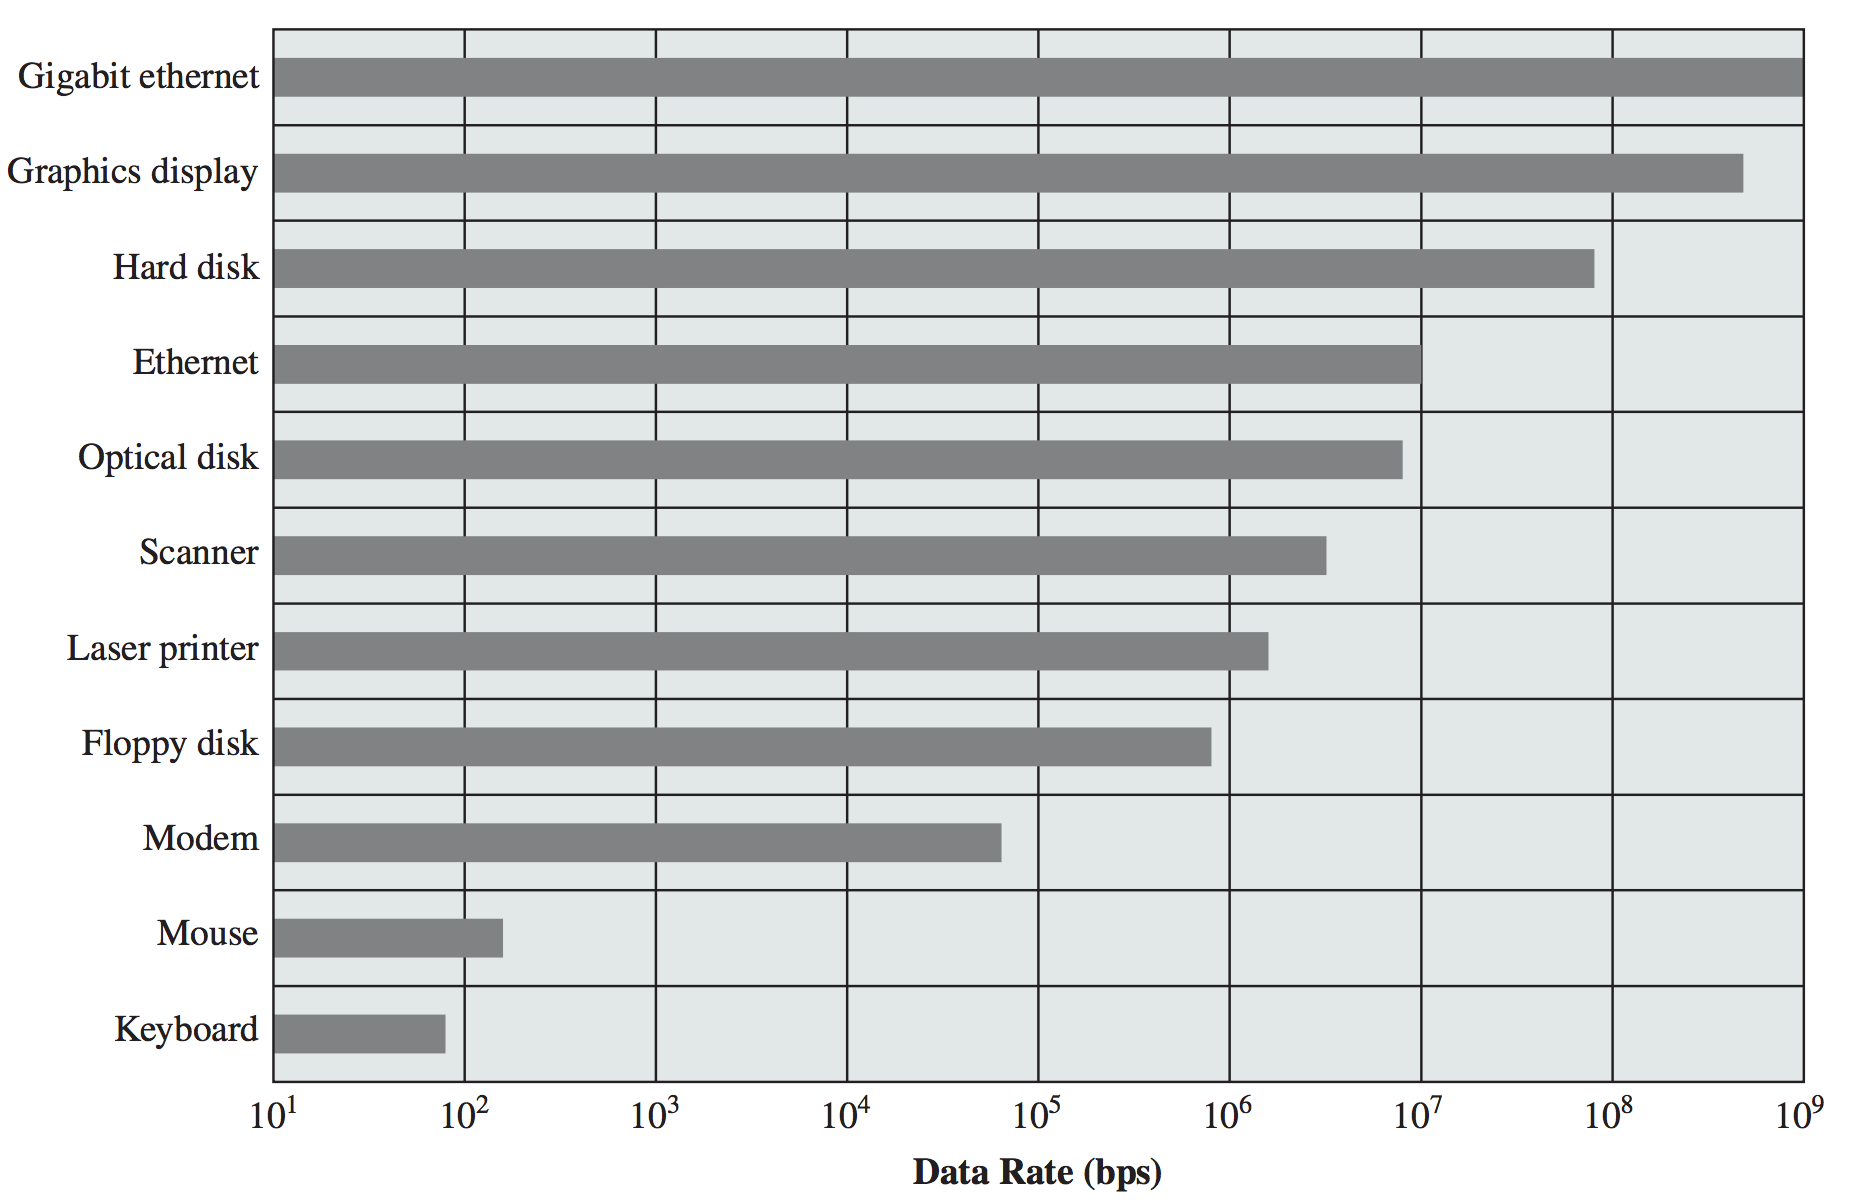
\includegraphics[width=0.75\textwidth]{images/io-device-rates.png}\\
	Typical I/O Device Data Rates~\cite{osi}.
\end{center}

We might like to think that USB has taken away some of the complexity, but that's just the way a device connects to the computer; managing the device itself is still as complicated as ever. All of the examples just listed in the previous paragraph can be connected via USB (Universal Serial Bus). And indeed, just because the computer and device have compatible physical connectors does not mean that the computer knows how to interact with the device. This can be kind of frustrating.

Disk I/O, when discussing magnetic hard disks, has a huge impact on system performance that it will receive its own discussion. But first, a little discussion about I/O in general.

\subsection*{Communication with Devices}
There are three ways, realistically, that we can communicate with a hardware device: polling, interrupts, and DMA (direct memory access). This isn't a hardware course, but I think we should review this topic at least a little bit before we go on. It's fair to say that these options are not all equally good; polling would be something we do because we must, not because it's efficient.

An I/O port represents the connection, and may typically have four registers: the data-in register (input), data-out register (output), status register, and control register~\cite{osc}. The control register is how the user or operating system gives commands to the device, and the status register tells us the current state of the device. Those aren't too exciting. 

The literature tends to refer to the main system as the ``host'', because the code that's interacting with the device could be the OS or it could be user-level code depending on the situation. So we'll use the word host.

\paragraph{Polling.} 
The most basic way to interact is polling, and as we've just discussed, it is the last choice but there might be the only choice. When a command is issued, the controller uses a bit to mark the device as ``busy'' during the time that the operation is taking place. When the operation is done, the bit is cleared. After that the OS can take the next action, whether that's reading the data requested or scheduling the next write or moving on from the operation to the next thing. 

This isn't super exciting, but it does work. The host has to check the state of the device repeatedly until the busy bit is cleared. It's not really efficient, because the CPU executes lots of instructions that are not doing useful work while it repeatedly reads the value of the busy bit. 

A first thought would be to change the logic a bit such that instead of tight polling, the host checks periodically rather than immediately. That does decrease the wasted CPU cycles, but has a risk that the data is lost because the host does not respond in time. If the data storage for the device itself is very limited, if the data currently ready is not retrieved fast enough, then the data might be overwritten by new data, causing some input to be lost~\cite{osc}.

\paragraph{Interrupts.}
Interrupts are something we've spent a ton of time talking about, but remember that this will operate on the basis of there being some sort of interrupt request line (hardware) and when the CPU sees the signal that indicates the presence of an interrupt, the interrupt handler is executed to deal with it~\cite{osc}. The interrupt handler will do whatever it's supposed to do and then clear the interrupt signal.

This description is fully correct, but overlooks some of the complexity around interrupts. For one thing, not all interrupts are equally important -- incoming phone call is not as urgent as a fire alarm. The other part is that interrupts should be something the CPU can (mostly) turn off it that makes sense. 

The interrupt approach helps to deal with the problem of not responding in time to the availability of data: when the interrupt is triggered, take the data from the device and put it in memory somewhere. This does not mean that the data has to be processed immediately, and it might actually be preferable to delay handling it until enough data has arrived. But as long as the data is in memory it won't get overwritten unexpectedly. 

\paragraph{Direct Memory Access.} 
Direct Memory Access or DMA is based on the idea that it's preferable to hand off some work from the CPU to a delegate, the DMA controller. The idea is that the DMA controller is given instructions about what to do: the operation to perform (either a read or write), the source, the destination, and how much data to be transferred. This can be efficient -- if copying data from, say, a USB drive to the hard drive, the data doesn't have to go to the CPU in between.

When the I/O operation is completed, the DMA controller will notify the CPU with an interrupt; but one thing that may not be obvious from the description is that the DMA controller might slow down the CPU a little bit because it's using the bus and that can make the CPU wait~\cite{osc}. That's still probably less than if it was an interrupt-based system. 

\subsection*{Application I/O Interface}
The use of DMA and interrupts are intended to increase the efficiency of the system, because we know that most devices are very slow when compared to the speed of the CPU and even memory~\cite{osi}. A lot of the efficiency gains, though, are based on what hardware is available so not necessarily something we can control when developing an operating system. Yes, the hardware is useless if the operating system does not use it, but the OS cannot compensate for the lack of a DMA module.

Ideally, when a general-purpose operating system is written, it will accept new devices being added to the system without editing/reinstalling/recompiling the code. Your experience with object oriented programming gives you some familiarity with the solution of how we should accomplish this goal. We want to abstract away the details of the hardware, to the extent we can, and provide a uniform \textit{interface} to interact with. 

In the very early days of operating systems, the hardware the computer shipped with was all the hardware it ever supported. If the vendor came out with a new module, they would have a new operating system update to introduce support for that device. This got to be unmanageable in the era of the IBM PC because anybody could create hardware and attach it via a standard interface. Relying on IBM or Microsoft or whoever your OS vendor was to implement support for a random piece of hardware was not realistic.

And from the operating system developer point of view, it's hard to argue. How are they to know what hardware devices exist, and even if they did, how they work? Some sort of standard interface only gets you so far. You can have one printer masquerade as another -- many years ago my parents had a Panasonic printer that you could tell the operating system was an Epson printer. That sort of works, but what about a new type of device or a device that is similar to an existing one but has some additional features or functionality?

Operating system developers thought they were very clever. They realized that they could shift the work to the hardware developers through a concept called \textit{device drivers}. The device driver plugs in to the operating system through a standard interface and tells the operating system a bit about the hardware and translates commands from the operating system to hardware instructions. Where this fell apart was the fact that hardware developers often made extremely poor drivers (whether this was due to inability or lack of caring is not clear).

The problem was exacerbated by a Windows design decision that device drivers would run in the system at the same protection level as the kernel. Some other operating systems have user-mode drivers, where possible (in Mac OS X and Linux systems, for example, there is the ability to have file system drivers in user space through a program called FUSE) or at an intermediate level between that of user space and the kernel. In any event, in Windows, if a device driver is unhappy with the current state of the system, contains a programming error, or encounters a situation it cannot handle, the driver can invoke a system call that brings up everyone's favourite feature: the Blue Screen of Death (BSOD).

Microsoft, rightly or wrongly, was blamed for a lot of those blue screens of death. If it appears after upgrading or patching the operating system, users blame the most recent thing changed, even if that's not what caused it. It also didn't help that the message said something about Windows has encountered a problem. That sounds like Windows is the one with the problem. 

Microsoft took two approaches to remedy this problem. One was to write and include in Windows a lot more device drivers. Including the drivers isn't too bad, but writing them yourself is painful. But user experience is key, and some effort invested into this probably does pay off. ``It's not my job'' is nice to say but sometimes getting the customer to sign the deal is more important than feeling right on principle.

The other approach Microsoft took was to introduce the static driver verifier, a complex piece of static analysis software used to test, at compile/build time, whether the driver will behave badly. Passing this test is required to get a sticker of approval from Microsoft to put on the box. So, the battle rages on about who is responsible for writing the drivers, unfortunately.

Device drivers, when they exist, connect into the kernel's I/O subsystem to mediate between the kernel's I/O subsystem and the hardware device controller. See the diagram:

\begin{center}
	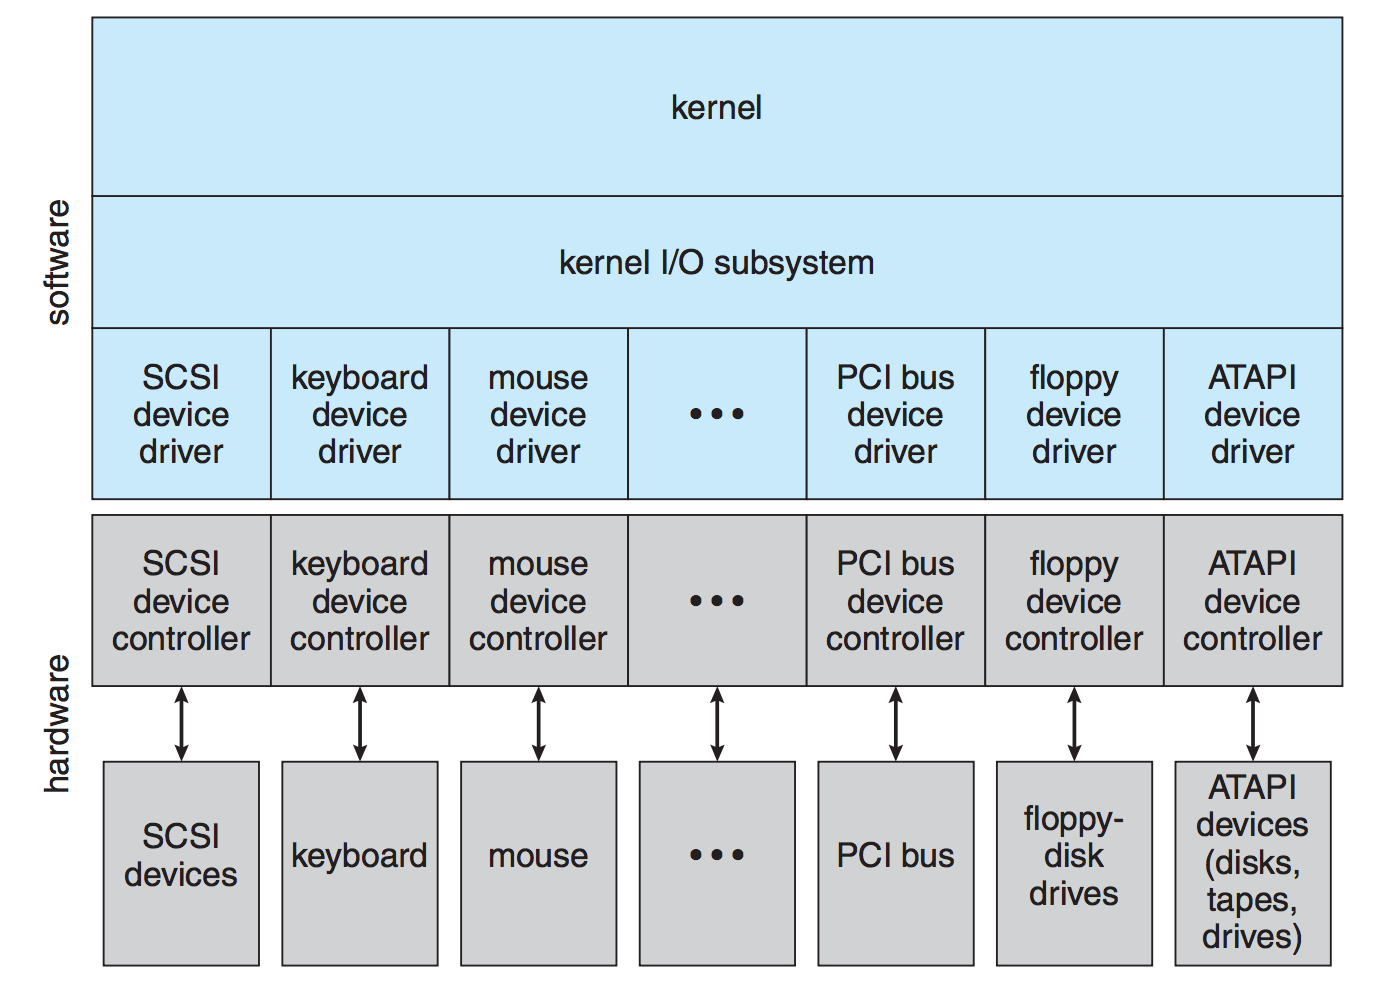
\includegraphics[width=0.65\textwidth]{images/kernel-io-structure.png}\\
	Kernel I/O structure, showing the placement of device drivers~\cite{osc}.
\end{center}

Abstracting away details of the hardware makes the job of the operating system developer easier: the interface provides a standard way of interacting with the hardware device. In Windows and Linux, for example, there exists another layer to add some more indirection between the OS and platform-specific hardware. It is called, obviously, the hardware abstraction layer. The HAL is supposed to make it easier to port the operating system to new hardware.


Unfortunately, every piece of hardware could be completely different. Even if the goal is just classifying devices based on similarity, devices can vary on numerous dimensions. Here's a list of a few examples from~\cite{osc}:

\begin{itemize}
\item \textbf{Data transfer mode}. A device may operate on a character level (transfer one character at a time) like a keyboard, or may operate on a block (group of bytes) all at once, such as a disk operating on a 4~KB block.
\item \textbf{Access method}. A device may allow only sequential access (that is, reading only the next element or piece of data or writing to the next location) such as a modem, or it could allow random access (reading from or writing to any point) as in a hard drive.
\item \textbf{Transfer schedule}. The schedule may be synchronous (transferring data with predictable response times) as in the case of reading from tape, or asynchronous (with unpredictable response times), such as awaiting a response that will come over the network.
\item \textbf{Dedication}. A device may be shareable (allows multiple concurrent threads) such as the speakers, or dedicated (allowing only one thread to use it at a time), such as a printer.
\item \textbf{Device Speed}. Recall the diagram from earlier showing the dramatic differences in transfer speeds.
\item \textbf{Transfer Direction}. Some devices are input only (such as a temperature sensor), other devices are output only (speakers), and some devices are capable of both (hard disk).
\end{itemize}

We would like to, as much as possible, keep the details above from the operating system, though devices will typically be grouped into a few categories so appropriate system calls can be issued. If a device is block-oriented, the OS should be issuing block read and write commands, not trying to do it one character at a time. Just for the sake of efficiency.

Operating systems also usually have an \textit{escape} system call that allows passing of a command directly from an application or the kernel to a device driver. This allows us to issue commands to a device that the OS designers have not thought of and created system calls for. The UNIX system call for this is \texttt{ioctl} (``I/O Control'') and it takes three parameters: a file descriptor indicating the hardware device (everything in UNIX is a file, remember), the command number (an integer), and a pointer to an arbitrary data structure (presumably \texttt{void*}) that has any necessary control information and data~\cite{osc}.


\subsection*{Block and Character I/O}

The block device interface is used for block devices such as hard disk drives. Any device will support \texttt{read} and \texttt{write} commands, and if it is a random-access device, it will have a \texttt{seek} command to jump to a specific block. An application usually accesses the hard disk through the file system, but going even one level lower, the OS can work on the hard drive using these two/three commands without being concerned with how that command is actually transmitted to the physical hardware.

We can abstract things a little bit further, from the perspective of the application developer, by having a memory-mapped file. Then, rather than using the block oriented operations directly, the application just writes to and reads from ``memory'' and the OS handles the behind-the-scene coordination to make writes go out to the correct block and read from the correct block.

A character-oriented device is something like the keyboard; the system calls are \texttt{get} and \texttt{put}. Libraries and other structures may exist to work on a whole line at a time (compare to, for example, the Java constructs for reading and writing files: the default streams are one character at a time, but if you want anything other than terrible performance, use a buffered reader which can read a whole line). This is a good match for input devices that produce data in small amounts and at unpredictable times, and perhaps for printers and sound output which operate naturally on a linear stream of bytes~\cite{osc}.

\subsection*{Network Devices}

Network devices are fundamentally different from those that are directly attached to the system. Thus, the \texttt{read}, \texttt{write}, and \texttt{seek} routines are not really appropriate. The model we are most familiar with from previous courses is the socket model. A socket is treated like a file, and at a basic level we can just ignore the details.

But we also learned about the \texttt{select} and \texttt{poll} functionality to support servers with multiple clients. That manages a set of sockets. Invoking this function returns information about what sockets have a packet waiting to be received and which are available for sending a packet. Proper use of \texttt{select/poll} eliminates polling and busy-waiting in a situation where delays are unpredictable (which is always the case with the network). Most likely, however, you remember that asynchronous I/O is difficult to manage. 

\subsection*{Spooling and Reservations}
A \textit{spool} is a buffer for a device, like a printer, that can serve only one job at a time. Unlike disk, where it might read for $P_{1}$ now and then write for $P_{2}$ immediately afterwards, a printer needs to finish a whole print job before it starts the next. Printing is the most obvious example, but it is by no means the only one. The operating system centralizes all communication to the printer and runs it through the spooling system. 

\subsection*{I/O Protection}
Recall from much earlier the idea of kernel mode and user mode instructions; some processor instructions are restricted such that only the OS can issue them (in kernel mode), otherwise it is an error (illegal instruction). We want all user accesses to I/O to be mediated through the operating system, so the OS can check to see if the request is valid. If it is, allow it to proceed; otherwise terminate the process with an error. This helps minimize errors and problems where people do bad things like cancel another process's request so theirs can go first. Our typical tradeoff: increased safety in exchange for reduced performance.

In certain circumstances, for performance reasons, we might want to allow direct access. In the case of a game, for example, we want to allow the game to work directly on the graphics card's memory (despite the fact that it is an I/O device). Mediating every access through the kernel would result in unacceptably poor performance (which is to say, the other team would totally call us noobs). So a section of graphics memory, corresponding to a particular window on the screen, will be locked by the kernel to be accessible by the game's process~\cite{osc}.

\subsection*{Kernel I/O Data Structures}
The kernel must, as is rather obvious, keep track of what I/O devices are in use by which processes and the general state of the I/O device (``PC Load Letter''). The diagram below gives some indication of what the UNIX kernel structures are like for open files:

\begin{center}
	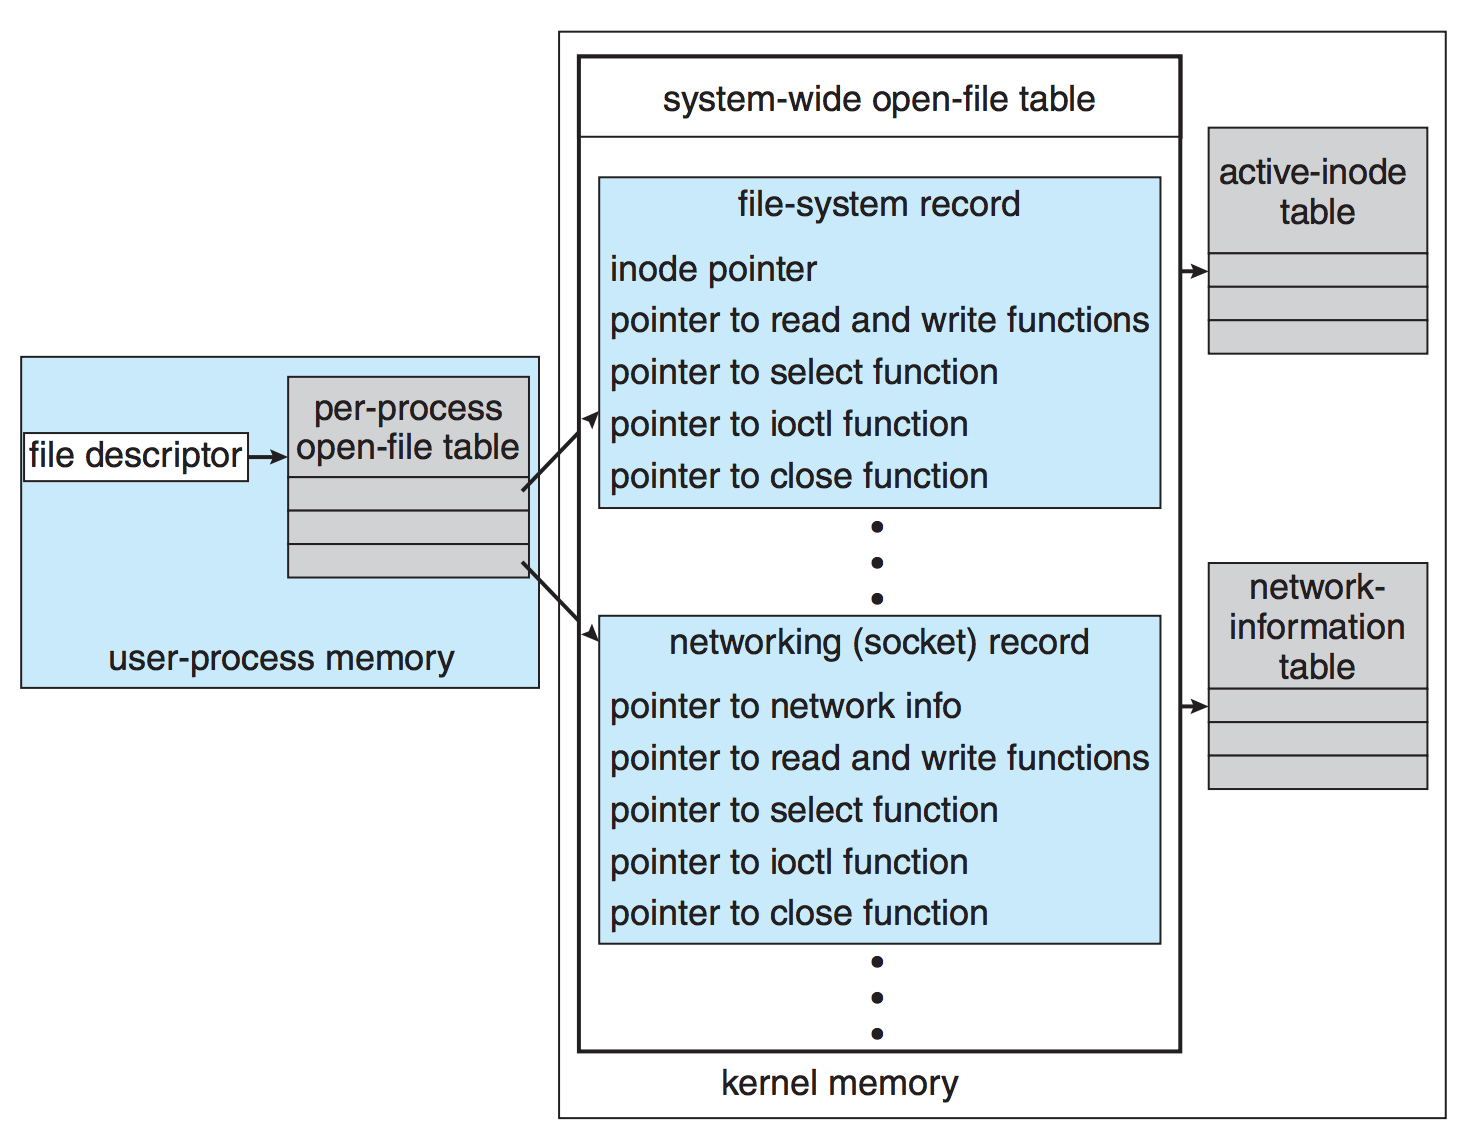
\includegraphics[width=0.7\textwidth]{images/unix-io-kernel.png}\\
	The UNIX structures to manage I/O~\cite{osc}.
\end{center}

This now explains why, if you print a file descriptor number and you see something like 3 or 4 -- that's the index into the per-process file table, which itself just references the system open-file table.

\bibliographystyle{alphaurl}
\bibliography{350}


\end{document}